\section{Représentation d'un atome (3 points)}\label{ex:avions}

Les avionneurs utilisent un métal léger pour construire certains avions. Un atome de ce métal, a pour numéro atomique Z = 13.

\begin{questions}
	\question[1] Combien cet atome possède-t-il de charges positives et négatives ?
	
	\begin{solution}
		Cet atome possède 13 charges positives et 13 charges négatives.
	\end{solution}
	
	\question[1] Dessiner cette particule en représentant un électron par un point rouge et le noyau par un point bleu.
	
	\begin{solution}
		\begin{center}
			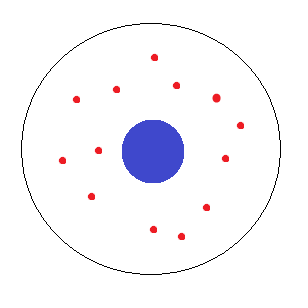
\includegraphics[scale=0.5]{img/al}
		\end{center}
	\end{solution}
	
	\question[1] Quel est le nom de ce métal ?
		\begin{solution}
			Ce métal est l'aluminium.
		\end{solution}
	
	\question[1] Combien cet atome possède-t-il de protons ?
	\begin{solution}
		Il possède 13 protons.
	\end{solution}
\end{questions}